\documentclass[aps,pra,10pt,twocolumn]{revtex4-2}
% revtex4-2 = version 2 of the review text class
% aps       = American Physical Society (society type)
% pra       = Physical Review A (journal type)
% 10pt      = font size
% twocolumn = true

\usepackage{silence} % NB: put *before* package you want to silence
\WarningFilter{caption}{Unknown document class} % Caption package does not support revtex4

\usepackage{times} % Times New Roman

\usepackage[a4paper, left=1.85cm, right=1.85cm,top=1.85cm, bottom=1.85cm]{geometry}

% Defines caption font size as 9pt and caption title bolded
\usepackage[style=base, font=small, labelfont=bf]{caption}
\usepackage{subcaption}

\usepackage{graphics,graphicx,epsfig,ulem}  % Graphics package
\usepackage{amsmath} 						% Maths package

\usepackage{siunitx} % SI units, alignment in tables

\usepackage{lipsum}
\usepackage[british]{babel} % British date system

\usepackage{multirow} % Multirow cells in tables
\usepackage{booktabs} % Nice table separators

\usepackage{hyperref} % For hyperreferences


% Customise date to preferred format
\usepackage{etoolbox}
\makeatletter
\patchcmd{\frontmatter@RRAP@format}{(}{}{}{}
\patchcmd{\frontmatter@RRAP@format}{)}{}{}{}
\renewcommand\Dated@name{}
\makeatother

\usepackage{fancyhdr}
\pagestyle{fancy} % Insert header
\renewcommand{\headrulewidth}{0pt}
\lhead{L.\ Kirby}
\rhead{Towards the automatic arrangement of music via quantum annealing}

\def\bibsection{\section*{References}} % Defining bibsection
 
\begin{document}

\title{Towards the automatic arrangement of music via quantum annealing}
\author{L.\ Kirby} % Author
\affiliation{Durham University} % Subtitle
\date{Submitted: \today{}} % Date

\begin{abstract}              

\lipsum[1]

\end{abstract}

\maketitle

\thispagestyle{plain} % Produces front page number

\section{Introduction} 

Music is often seen as a very human endeavour. For centuries, only skilled musicians could compose and perform such sequences of sound that would be considered art. Some would go one step further and adapt previously composed pieces for practical or artistic reasons, whether that be in terms of instrumentation, medium, or style, to create an \textit{arrangement}. One of the most famous examples of this is \textit{Pictures at an Exhibition}, a piano suite written by Modest Mussorgsky, but more commonly known for its orchestral arrangement by Maurice Ravel.
Traditionally, the arrangement of music is a complex process that requires a deep understanding of musical theory, structure, and style. Composers use their creativity and intuition to create a piece that is both musically interesting and emotionally engaging whilst still remaining faithful to the source material—a challenging and often time-consuming process. Perhaps it is unsurprising, then, that there has been interest in automating this process.

One of the earliest examples of this can be seen in the \textit{Musikalisches Würfelspiel} (``musical dice game'') system popular in the 18th century. The roll of dice would determine the order of pre-composed musical phrases, allowing for the creation of new music without the need for a composer. This system was engaged by the likes of Bach and Mozart, although fell out of fashion the following century.
The introduction of computers in the 20th century allowed for more sophisticated methods of music arrangement. Composers could now transpose and manipulate musical parts digitally, without the need to calculate parts by hand. Moving into the 21st century, more advanced techniques such as genetic algorithms and neural networks have been used to arrange music, with varying degrees of success. However, these methods are limited by the complexity of the problem and the need for extensive training data.

The field of quantum computing has its foundations as early as the 1980s, with the suggestion that hardware following the laws of quantum mechanics could be more efficient than its classical counterpart. Since then, two types of quantum computers have been developed: gate-based and annealing. Gate-based quantum computers, such as those developed by IBM and Google, use quantum gates to manipulate qubits and perform calculations. Quantum annealers, such as those developed by D-Wave, use quantum fluctuations to find the global minimum of a given function. Each are suited to solving different classes of problems, with gate-based computers being more versatile and annealers being more efficient for certain optimisation problems. 

The combination of quantum computing and music is a relatively new field, but one that has shown promise. Quantum computers have been used to write melodies \cite{arya_music_2022}, harmonies \cite{freedline_algorhythms_2021}, create synthesisers \cite{miranda_hello_2020}, and compose remixes \cite{miranda_impossible_2022}, using a mixture of gate-based and annealing methods. However, most of these efforts have been directed at music \textit{composition}, that is, the generation of entirely new sequences and sounds, rather than music \textit{arrangement}. Quantum computers, specifically quantum annealers, have the potential to solve complex optimisation problems that are intractable for classical computers, and music arrangement is one such problem.

Quantum annealers are particularly well-suited to solving a class of problems known as NP-hard, defined in the field of computational complexity as a optimisation problems where the time taken to find a solution scales exponentially with the input size. A well-known example of an NP-hard problem is the travelling salesman problem, where the goal is to find the shortest route that visits a set of cities exactly once. This problem is difficult to solve because the number of possible routes grows rapidly with the number of cities. Quantum annealers have been shown to be effective at solving NP-hard problems, and have been used to find solutions to a variety of optimisation problems, such as protein folding [CITE], financial portfolio optimisation [CITE], and traffic flow optimisation [CITE].

This paper will focus on a subset of arrangement known as \textit{reduction}—taking a score written for a large number of parts and reducing it to a smaller number of parts, whilst still retaining the musicality and structure of the original. This is a common task in music production, where a piece written for a full orchestra may need to be arranged for a smaller ensemble, such as a string quartet. This forgoes the need to generate new music, as all notes in the arrangement are taken from the original score, and is more readily available to analyse as an optimisation problem. In this study, music arrangement is formulated as an NP-hard optimisation problem, and solved via quantum annealing to produce a valid reduction.
\clearpage

\section{Theory}

Annealing, in metallurgical terms, is the process of heating and cooling a material to alter its physical properties. The cooling stage is typically slow, allowing particles to arrange themselves into regular lattice structures, making the material softer and less brittle \cite{oed_annealing_2024}. In the context of quantum computing, quantum annealing is the process of slowly changing a quantum system from one Hamiltonian to another. Much like its metallurgical counterpart, this computational technique allows the system to settle into a more useful final state.

The typical time evolution of a quantum annealer looks like
\begin{equation}
    H(t)=\left(1- \frac{t}{T}\right)H_0 + \frac{t}{T}H_p \,,
    \label{eq:time-evolution}
\end{equation}
where $H_0$ is the initial ground state, allowed to evolve to a second state $H_p$ across time $T$. If this is done adiabatically, with a sufficiently large $T$, the system will remain in the ground state of $H(t)$, and therefore end in the ground state of $H_p$ at time $T$. This is the principle of quantum annealing.

The main use of quantum annealing is to solve combinatorial optimisation problems, which are problems that require the minimisation of a function over a discrete set of variables. If we prepare $H_p$ such that its ground state encodes the solution to the optimisation problem, then as long as $H_0$ and $H_p$ do not commute, the solution will be given at the end of the annealing process.

In order to encode a problem, $H_p$ Hamiltonians take the form of an Ising spin glass, a random arrangement of magnetic dipole moments that can be in one of two states, typically spin-up ($+1$) or spin down ($-1$). A spin glass with a vector $s$ of $N$ spins takes the form
\begin{equation}
    H(s) = -\sum_{i<j}J_{ij}s_i s_j - \sum_{i=1}^{N}h_i s_i
    \label{eq:ising}
\end{equation}
where $J_{ij}$ are the coupling strengths, and $h_i$ are the field strengths. The quantum case can be expressed as
\begin{equation}
    H_p = H(\sigma^z)
\end{equation}
where we have replaced the spins with Pauli matrices. This is the \textit{Ising model}. The discrete variables are now \textit{qubits}—binary variables like their classical counterparts, but existing in a superposition of the two states until measurement. The ground state is prepared with the Hamiltonian 
\begin{equation}
    H_0 = -h_0\sum_{i=1}^{N}\sigma_i^x
\end{equation}
which is an equal superposition of all possible states in the eigenbasis of $H_p$ \cite{lucas_ising_2014}.

The mapping of a logical problem to an Ising model is called \textit{embedding}. Problems are formulated in an analogous way to a spin glass via a QUBO (quadratic unconstrained binary optimisation). A QUBO takes the form of a function $f(x)$ to be minimised, and is represented by
\begin{equation}
    f(x)=\sum_{i<j}Q_{i,j}x_ix_j + \sum_iQ_{i,i}x_i
    \label{eq:QUBO}
\end{equation}
where $x$ is a vector of binary variables (taking the values $0$ or $1$), and $Q$ is an $N\times N$ upper-diagonal matrix of real weights. The off-diagonal $Q_{i,j}$ terms are known as quadratic coefficients, and diagonal $Q_{i,i}$ terms as linear coefficients. As its name suggests, a QUBO can only include terms up to the second power, restricting coupling to pairwise interactions just as the Ising model.
This form can easily for transformed to an Ising model using
\begin{equation}
    s_i = 2x_i - 1 \,.
    \label{eq:qubo-ising}
\end{equation}

Once a QUBO has been expressed, it can be sent to a quantum processing unit (QPU) to be solved. The graph architecture of these units allows the mapping of problem QUBOs to physical qubits, with linear terms ($x_i$) as nodes and quadratic terms ($x_ix_j$) as couplers. An embedded system can then be prepared in its initial ground state, and allowed to evolve adiabatically to its final state to obtain the solution.

However, the topology of these graphs often doesn't allow an exact one-to-one mapping; it may be the case that the problem requires a qubit to have more couplers than physically allowed. The solution to this is the introduction of chains. A chain of physical qubits can act like a single logical variable, allowing more connections. The chain strength determines how strongly the chain is coupled, enforcing all qubits within the chain to have the same value. Chain strength is an important parameter that can affect the quality of solutions: if it is too weak, a final state may include chain breaks that return an infeasible solution; if it is too strong, it can overpower the other terms in the QUBO.

\begin{figure}[h]
    \centering
    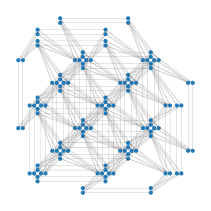
\includegraphics[width=\linewidth]{../Figures/pegasus.pdf}
    \caption{A graph of 144 qubits in a D-Wave QPU, using their Pegasus topology. Qubits are represented by nodes, and couplers by edges.}
    \label{fig:pegasus}
\end{figure}

The qubits and their couplers define what can be seen as an energy landscape. Different combinations of qubit spins will have different energies, with the lowest energy state being the solution to the problem. A solver (or ``sampler'') attempts to characterise the shape of the energy landscape using a random range of input, and returns a number of samples with the lowest energy states. Note that the ``true'' ground state cannot be guaranteed; it could be part of the returned sampleset, or may not even be found at all. It is the parameters of the annealing process that can reduce local minima and increase the likelihood of finding the ground state.

The full embedding process is often handled entirely by the QPU, done ``on the fly'' each time a problem is submitted. Fixed embeddings can be specified, but these require a priori knowledge of the specific QPU architecture. 

\section{Problem formulation}

Previous approaches to the automatic arrangement of music rely on neural networks [CITE] or recursive classical algorithms [CITE]. However, these methods are limited by the complexity of the problem and the need for extensive training data. In this study, we propose a new approach to the automatic arrangement of music by applying quantum annealing.

It has been shown that the automatic arrangement of music can be formulated as a combinatorial optimisation problem: given a set of musical phrases, each phrase can be assigned a binary variable and formulated into a boolean satisfiability (SAT) problem, with variables assigned to clauses according to their compatibility. A valid solution would be an assignment of values such that the boolean expression is satisfied, corresponding to phrases included in the final arrangement \cite{moses_computational_2016}. Phrases are chosen as the smallest unit of music instead of notes to best preserve important melodic lines and harmonies, which may sound dissonant if split up.

This paper focuses on the reduction of polyphonic (multi-part) music to a single monophonic part, where only one note can be played at a time. A reduction of this form would be relevant for arranging a string quartet for solo violin, for example, whilst still retaining all the important elements from across the instrument parts. This problem can be solved using a reduction of the SAT problem known as the maximum independent set (MIS) problem \cite{lucas_ising_2014}. Consider a set of musical phrases, each represented by a node $x_i$ in a graph $G$, with nodes connected by an edge if the phrases overlap. The aim is to find the largest subset of nodes such that no nodes within the subset are connected by an edge—the phrases corresponding to these nodes form the final arrangement. A formulation of this sort ensures that the reduction remains strictly monophonic, as no two chosen phrases play at the same time.

The MIS QUBO takes the form
\begin{equation}
    f(x)=A\sum_{ij\in E}x_ix_j-B\sum_i x_i\,,
    \label{eq:MIS}
\end{equation}
where we take $x_i=1$ as the inclusion of that node in the solution set. The first term (penalty term) implements the independence constraint by increasing the energy by $A$ for each edge included, whilst the second term (objective term) is the quantity we are trying the minimise, the (negative) total number of nodes.

\begin{figure}[h]
    \centering
    \begin{subfigure}[b]{\linewidth}
        \includegraphics[width=\linewidth]{../Figures/toy-1.png}
        \caption{An example score of three parts, with each phrase coloured.}
        \label{fig:simple-excerpt}
    \end{subfigure}
    \par\bigskip
    \begin{subfigure}[b]{\linewidth}
        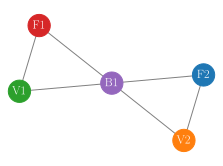
\includegraphics[width=\linewidth]{../Figures/toy_graph.pdf}
        \caption{A graph of the score, with the colour of each node corresponding to its phrase, and edges connecting overlapping phrases.}
        \label{fig:simple-graph}
    \end{subfigure}
    \caption{A toy example demonstrating the construction of the problem graph. It is trivial to see that the maximal independent set contains two nodes.}
    \label{fig:toy}
\end{figure}

To increase the quality of the final arrangement, this formulation can further be expanded to include weights on the nodes, which can be used to represent the ``musicality'' of the phrases. The MIS QUBO then becomes
\begin{equation}
    f(x)=A\sum_{ij\in E}x_ix_j-B\sum_i W_ix_i\,,
    \label{eq:weightedMIS}
\end{equation}
where $W$ is a vector of real weights. This way, fewer nodes may be chosen as long as it increases the overall perceived quality of the arrangement. 

% Physical implication of results
% Does code work? Comparison to literature, tests (IMPORTANT)

\section{Methods}

D-Wave Systems operates the first and only quantum annealer for public access [CITE]. All problems in this paper are run on the D-Wave Advantage quantum system, which uses their Pegasus architecture, with each qubit connected to 15 others. This allows for a high degree of connectivity, but also introduces the possibility of long chains, which can degrade the quality of solutions.
Since interaction with the D-Wave QPUs is handled in Python, the surrounding manipulation of music is also written in this way. The Python module \verb|music21| provides extensive resources for manipulating, translating, and creating music, allowing scores to be broken down and reconstructed as fit.

There are many formats that allow the digital manipulation of music, each with their own benefits—this study primarily uses MusicXML \cite{musicxml}. This format focuses on the representation of standard sheet music, describing musical notes, rests, and other symbols, as well as the structure of the music, such as the arrangement of notes into measures (bars), parts, and scores. It is widely supported by music notation software, allowing translation of music to graphic (PNG, PDF) and audio (MIDI) formats.

To begin processing, a MusicXML file of the original score is first interpreted by the program. Embedded metadata within the score allows it to be broken down into its constituent instrument parts, measures, and notes. Each note is represented by a vector of features, such as pitch and duration, as well as its position within the wider piece. [CAN ELABORATE HERE]

To construct the graph, each part needs to be split into a sequence of musical phrases. The approach taken here is the local boundary detection model (LBDM) [Cambouropoulos 2001] due to its easy implementation and good performance. The boundaries segmenting a musical line into phrases are identified using the degree of change between successive notes; larger differences between notes would show an increased likelihood of a boundary. Boundary strengths are calculated over two parameters, pitch and inter-onset interval (IOI), which is the difference between the starts of two notes. This is chosen over note duration as it is often more noticeable to the listener [CITE]. The strength at note $i$ with parameter $x_i$ is given by
\begin{equation}
    S_i=x_i\times (r_{i-1, i} + r_{i, i+1})
    \label{eq:boundary-strength}
\end{equation}
where $r_{i, i+1}$ is the degree of change of a parameter between notes $i$ and $i+1$ and given by
\begin{equation}
    r_{i, i+1}=\frac{|x_{i}-x_{i+1}|}{x_{i}+x_{i+1}} \,.
    \label{eq:degree-change}
\end{equation}
In this way, a note with a high boundary strength would signal the start of a new musical phrase. Each parameter's strength is normalised to the range $[0,1]$ according to the set of all strengths $S$ via
\begin{equation}
    S_i'=\frac{S_i-\min(S)}{\max(S)-\min(S)}
    \label{eq:normalisation}
\end{equation}
Finally, to find the total boundary strength, the strengths of each parameter are summed with a weighting, using weights derived by trial-and-error ($0.3$ for pitch and $0.6$ for IOI) [CITE]. If a note's total boundary strength surpasses a specified threshold, it is considered a boundary. Boundaries are always taken at the beginning and end of a part.

Once a list of boundaries is identified, the phrases are extracted by taking all the elements between subsequent boundaries. Each phrase is labelled according to the part it belongs to and its index within that part, allowing the phrases to be easily referenced and reconstructed into a new score once the optimisation is complete.

In order to construct the graph, each phrase is checked against every other phrase for an overlap in time. Phrases are then represented by nodes, with edges connecting phrases that overlap. The phrase nodes can be assigned a weighting based on their entropy. The entropy of a phrase can be seen as how much musical information it contains, with a higher entropy indicating a more complex phrase. Maximisation of phrase entropy can be used to create richer arrangements. For a discrete random variable $X$ with a probability distribution $P(X)$, the Shannon entropy is defined as
\begin{equation}
    H(X):=-\sum_i P(x_i)\log_2 P(x_i)
    \label{eq:entropy}
\end{equation}
where each $x_i$ is a possible value of $X$. In this context, the random variable is a musical note, considering its possible values both in terms of pitch and rhythm.

Pitch entropy is calculated by considering the distribution of pitches in a phrase. The probabilities of each pitch $x_i$ can be found by
\begin{equation}
    P(x_i)=\frac{n_i}{N}
    \label{eq:pitch-prob}
\end{equation}
where $n_i$ is the number of times pitch $x_i$ appears in the phrase and $N$ is the total number of notes in the phrase. A phrase with a greater variety of pitches (and thus greater entropy) will likely be more "interesting" in the final arrangement.

Rhythm entropy is calculated in a similar way, but instead of considering the duration of notes, the inter-onset interval (IOI) is used instead. This is also calculated using Eq.\ \ref{eq:pitch-prob}, but instead considering $x_i$ as possible IOI values.
The total entropy of a phrase is then the sum of the pitch and rhythm entropies.

Once the graph is formed, the weighted MIS QUBO can be constructed via Eq.\ [EQUATION] and sent to the D-Wave QPU to be solved. The solutions returned are sets of phrases that are compatible with each other and form the final arrangement. These are then reconstructed into a new object which can be translated into sheet music or audio.

% TODO: Make this list of phrases selected? With their entropies?
\begin{table}[ht] % Table environment specifies caption, label, location
    \caption{Summary of frational changes to best-fit parameters due to electron energy density and electrostatic corrections.}
    \label{tab:corrections}
    \setlength{\tabcolsep}{12pt} % Column spacing
    \renewcommand{\arraystretch}{1.5}
    \begin{tabular}{c|c|c|c} % S aligns to decimal point
        \toprule
        \textbf{Correction} & $|\Delta A|/A$ & $|\Delta B|/B$ & $|\Delta q|/q$\\
        \midrule
        $\varepsilon_\mathrm{elec}$ & 0.026 & 0.0031 & 0.0442 \\
        $p_c$ & 0.009 & 0.0114 & 0.0005 \\
        \bottomrule
    \end{tabular}
\end{table}

\section{Results}

The method was tested on an excerpt of String Quartet No.\ 10 in E-flat major, Op.\ 74, by Ludwig van Beethoven, nicknamed the ``Harp'' quartet. This was chosen due to its relatively simple structure and smaller instrumentation, making it easier to identify and arrange the musical phrases. Fig.\ \ref{fig:excerpt} shows the first 13 measures of the original score.

Phrases identified using the LBDM model are shown in Fig.\ \ref{fig:phrases}, alongside their calculated entropies according to Eq.\ \ref{eq:entropy}. A graph representation of the phrases can be seen in Fig.\ \ref{fig:graph}, with the nodes representing the phrases and the edges connecting overlapping phrases. Many of the nodes form cliques of three or four vertices, that is, each node of the subset is connected to every other node. This can be expected, as often musical phrases across instruments will occur simultaneously, especially in small ensemble music such as this. Notably, there are also two disjoint cliques, which can be seen as distinct musical ideas that are separtated by rests from the other phrases (for example, the first two measures of the piece). A non-negligibile number of phrases are calculated to have zero entropy—these are phrases identified as only having one note, and thus no variety in pitch or rhythm.

\begin{figure}[h]
    \centering
    \includegraphics[width=\linewidth]{../Figures/boundary_offset.pdf}
    \caption{Boundary strengths for each note of the viola part, calculated using Eq.\ \ref{eq:boundary-strength}. The dashed line shows the threshold value used ($0.4$). Notes above the threshold value are considered as boundaries for phrases.}
    \label{fig:boundary-strengths}
\end{figure}

\begin{figure}[h]
    \centering
    \includegraphics[width=\linewidth]{../Figures/problemGraph.pdf}
    \caption{The representation of Fig.\ \ref{fig:phrases} as a graph. The nodes are the identified musical phrases, with edges connecting them if they overlap. The entropy of each phrase is represented by the colour of the node.}
    \label{fig:graph}
\end{figure}

After submitting a QUBO calculated using Eq.\ \ref{eq:weightedMIS}, the D-Wave QPU returned a sampleset of solutions, which can be seen in Fig.\ \ref{fig:histogram}. Many solutions had the same energy but used slightly different combinations of phrases to make the maximal independent set; this degeneracy is likely due to the high number of cliques, which only allows one node of the subset to be picked, and phrases with zero entropy, which do not change the final energy when interchanged. One of the lowest energy solutions can be seen in Fig.\ \ref{fig:solution}, with the nodes selected by the QPU highlighted. In this solution, none of the nodes are connected by edges, providing a valid arrangement. The musical score of this solution is shown in Fig.\ \ref{fig:arrangement}.

\begin{figure}[h]
    \centering
    \includegraphics[width=\linewidth]{../Figures/histogram.pdf}
    \caption{A histogram of the solutions returned by the QPU, over 1000 total reads. Solutions with energies above zero are omitted.}
    \label{fig:histogram}
\end{figure}

\begin{figure}[h]
    \centering
    \includegraphics[width=\linewidth]{../Figures/solutionGraph.pdf}
    \caption{The graph of Fig.\ \ref{fig:graph} but with the nodes selected by the QPU highlighted. In this solution, none of the nodes are connected by edges, providing a feasible arrangement, which can be seen in Fig.\ \ref{fig:arrangement}.}
    \label{fig:solution}
\end{figure}

\begin{figure*}[h]
    \newcommand{\subfigurewidth}{0.9\linewidth}
    \centering
    \begin{subfigure}[b]{0.5\linewidth}
        \includegraphics[width=\subfigurewidth]{../Figures/excerpt-1.png}
        \caption{Original excerpt.}
        \label{fig:excerpt}
    \end{subfigure}\hfill
    \begin{subfigure}[b]{0.5\linewidth}
        \includegraphics[width=\subfigurewidth]{../Figures/selected-1.png}
        \caption{Selected phrases from solving the MIS problem.}
        \label{fig:selected}
    \end{subfigure}\hfill
    \par\bigskip
    \begin{subfigure}[t]{0.5\linewidth}
        \centering
        \includegraphics[width=\subfigurewidth]{../Figures/arrangement-1.png}
        \caption{Final arrangement.}
        \label{fig:arrangement}
    \end{subfigure}
    \caption{The beginning of String Quartet No.\ 15 in A minor, Op.\ 132, by Ludwig van Beethoven, reduced to a single part.}
    \label{fig:results}
\end{figure*}

\clearpage

\section{Conclusions}

It is clear that this method works for the excerpt shown here; future work would include testing this process on a wide range of pieces from different musical styles.

The MIS formulation works well for reducing a score into a single polyphonic part, as the inclusion of a phrase within the final arrangement has a direct match to the binary variables used. However, a more useful application would be the ability to reduce a score to any number of parts, whether that be multiple monophonic instruments (e.g.\ string quartet) or a polyphonic instrument (e.g.\ piano). One formulation that could solve this would be "colouring", that is, colouring each node of the graph such that no two nodes of the same colour are connected by edges. In this case, each colour would represent a monophonic part, and the set of colours combined would represent the final instrumentation.

One advantage this method has over classical algorithms is that no training data is needed. Genetic and deep learning approaches require refinement of their models on large datasets, using considerable time and resources. Due to the required constraints, the QPU will (mostly) always provide a feasible solution, without any knowledge of previous arrangements.

Another benefit is the solve time. For 1000 reads, the D-Wave QPU access time averages at $163\,\textrm{ms}$

Although it can be argued that music cannot be objectively "scored", nonetheless, the quality of the produced arrangements needs to be judged in some way. One suggestion is that the "goodness" of music can only be measured via a Turing-like test, where human subjects are presented with a selection of both human- and computer-generated scores, and asked to categorise them \cite{pearce_towards_2001}. To this extent, a good measure of the arrangements produced by this method would be to compare them against popular arrangements of the same score composed by human professionals, via a series of blind trials. If the participants fail to identify the computer compositions from the human ones more often than random chance, then it can be said that the generated arrangements are of sufficiently good quality.

\nocite{*}
\bibliographystyle{unsrt}\bibliography{interim}

\clearpage

\onecolumngrid % Puts summary into single column

\section*{Scientific Summary for a General Audience}

\lipsum[1]

\end{document}